%!TEX root = ../template.tex
%%%%%%%%%%%%%%%%%%%%%%%%%%%%%%%%%%%%%%%%%%%%%%%%%%%%%%%%%%%%%%%%%%%
%% sdn.tex
%% NOVA thesis document file
%%
%% Chapter with introduction
%%%%%%%%%%%%%%%%%%%%%%%%%%%%%%%%%%%%%%%%%%%%%%%%%%%%%%%%%%%%%%%%%%%

\typeout{NT FILE sdn.tex}%

\chapter[Software Defined Networking]{\acrlong{sdn}} % (fold)
\label{cha:sdn}


% introduction
\gls{sdn} is a networking paradigm that simplifies network management and promotes innovation through software-based approaches, rather than traditional hardware-based configurations. \gls{sdn} has the potential to shape the future of the Internet and is therefore often referred to as a "radical new idea in networking". \cite{nunes_survey_2014}
\gls{sdn} dates back to the 2000s, and its concepts can be traced as far back as the 1990s \cite{feamster_road_2013}, so this technology is not exactly new. The core ideas and motivations behind \gls{sdn} have been worked on and evolved over the past thirty years, with several previous efforts already being undertaken to promote network programmability\cite{feamster_road_2013}. Even though it is not the first, \gls{sdn} is considered the most promising as its uniqueness stands from providing programmability while offering to greatly simplify network devices. \cite{xia_survey_2015} 

In 2011, the Open Networking Foundation (ONF) consortium was founded with support from major players in the technology industry, including Google, Facepeterson_software-defined_2021, and Microsoft. ONF develops open standards for \gls{sdn} technologies to promote the \gls{sdn} vision. It is currently the leading consortium in this field. \cite{noauthor_open_nodate} 

The information in this paper on \gls{sdn} is largely supported by the peterson_software-defined_2021 \cite{peterson_software-defined_2021}, authored by leading researchers in the field and cited by the ONF itself.

Before delving deeper into this topic, it is worth emphasizing that \gls{sdn} is an approach to networking, rather than a point solution, so while some of the most important and widely adopted technologies will be mentioned in this chapter, they should be viewed as an attempt to achieve the \gls{sdn} vision.


% SDN definition
\section[SDN definition]{\gls{sdn} definition}

% traditional networks comparison
Traditional networks have a highly decentralized structure, which was essential for the early Internet to achieve high network resiliency \cite{kreutz_software-defined_2015}. As a consequence, Internet devices are vertically integrated, meaning the network control logic is directly coupled to the underlying forwarding hardware. This leads to routing decisions being made by complex programs running on each device through the definition of low-level policies. \cite{bifulco_survey_2018}

For a long time, researchers and developers have acknowledged that changes in the way the Internet works, nominally in its structure, were necessary to simplify and automate network management. These changes came to take place as the technology known as \gls{sdn}, which breaks down the vertical integration of devices.  \cite{thyagaturu_software_2016}

 	% main principles
\gls{sdn} technology nowadays is rather an umbrella term, as many different researchers have their own nuanced definition arising from different levels of implementation of the same \gls{sdn} vision. Such discrepancies in the \gls{sdn} definition is acknowledge by \cite{livro} and can be visualized in \cite{feamster_road_2013} \cite{thyagaturu_software_2016} \cite{nunes_survey_2014} \cite{bifulco_survey_2018}.
The early \gls{sdn} proposal stood on three main principles, which are still relevant to this day and are as such:

\begin{itemize}
% Decoupling 
	\item First and foremost this technology is characterized by the decoupling of the control plane from the data plane. 

\begin{figure}
    
\end{figure} 

    The control plane can be considered as the “brain” of the network. It is responsible for commanding forwarding operations in the whole network, making decisions on how to handle network traffic.  

    The data plane is the remaining forwarding hardware that follows the commands set by the control plane. By removing the decision making components from network devices, it makes them simple forwarding devices.

    Network intelligence is thus removed from individual devices, transforming all networking equipment into simple packet-forwarding switches.
% Centralization

	\item The second principle of \gls{sdn} requires a logically centralized control plane that manages the data plane through well-defined APIs. This means that a single entity, commonly known as the controller, oversees all of the network. 
% Programmability

	\item Lastly, the controller must have the power to control network behavior through the programming of network functions. \gls{sdn} must allow software developers to harness and utilize network resources similarly to computing resources and storage. 
\end{itemize}

% Considerations
To sum up, and as can be seen in Figure X, \gls{sdn} requires the decision making elements of a network are decoupled from forwarding devices and logically centralized in a single entity, which is a programmable controller. 

\begin{figure}
	\centering
	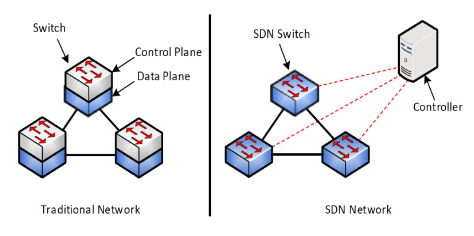
\includegraphics{Chapters/Figures/SDNs/sdn_vs_legacy.png}
	\caption{Traditional network view Vs \gls{sdn} Network view}
	\label{fig:sdn_vs_legacy}
\end{figure}
%\cite{object_scalable_nodate}

As a consequence from these principles, an \gls{sdn} switch can function as any traditional Internet device, such as a router, switch, firewall, network address translator, or even a combination of these. 

% More recent developments
These three principles remain relevant today and form the de facto definition of \gls{sdn}. However, in recent years, new efforts have been made beyond this initial definition to further fulfill \gls{sdn}'s original goal. These efforts aim to increase programmability to the data plane, allowing network operators to fully customize all traffic in the network.

% next gen SDN
Some articles refer to these recent efforts as next generation \gls{sdn} \cite{liatifis_advancing_2023} \cite{sofia_shaping_2024}, while predicting further and further coupling of \gls{sdn} with network virtualization.

% Network Virtualization	
Being one of the first use cases found for \gls{sdn}, Network virtualization traces its roots to the 90’s, around the same time the idea of programmable networks was surging. \cite{kreutz_software-defined_2015} \cite{feamster_road_2013} 

Network virtualization enables the creation of network topologies decoupled from the physical topology. This allows multiple virtual networks to share the underlying physical infrastructure, functioning seamlessly over the same physical network. \cite{thyagaturu_software_2016} The advantage of network virtualization is that it allows each individual virtual network to be simpler than the real network topology, granting increased flexibility. 

Network virtualization and \gls{sdn} are two distinct technologies that do not require each other to exist. However, \gls{sdn} technology enables network virtualization, effectively creating a mutually beneficial relationship between the two that has grown much closer over the years\cite{feamster_road_2013}.

% 2 phase SDN
Another way to interpret these recent \gls{sdn} developments is to divide efforts into two phases. In the first phase the control plane is centralized and opened for operators, for more network control, and in the second phase the data plane is opened, allowing network operators to better control packet processing in the network. 

“Fig. 1. Evolution of networks: left image depicts a traditional networking element, middle image depicts an OpenFlowbased network element and right image depicts a P4-based networking element.” (liatifis_advancing_2023, p. 1864)

In reality, \gls{sdn} implementations may mean more or less than the original definition depending on the involved stakeholder that is deploying the technology, as each network operator has the freedom to fulfill this view however they wish. \cite{peterson_software-defined_2021}

From this, and from the fact that \gls{sdn} is a disruptive technology, hybrid solutions that aim to harness some of the \gls{sdn} benefits while maintaining the status quo in the industry have appeared. These solutions mainly appear as attempts from manufacturers to maintain their established business models. \cite{peterson_software-defined_2021}

Lastly, it should also be noted phase 1 \gls{sdn} was largely impelled forward by Openflow, while phase 2 is marked by the development of P4. Both these technologies will be further discussed in Section \ref{}.


% Advantages of SDN
\section[Motivation behind SDN]{Motivation behind \gls{sdn}}

The Internet currently faces numerous challenges, ranging from expensive, complex network structures that are difficult to manage and optimize, to significant barriers to the development and deployment of new network design ideas. The networking research community and industry have recognized that these challenges require a novel approach to network structure. \gls{sdn} promises to solve these problems by providing programmability, flexibility, improved performance, and support for implementing and testing new network ideas.

This section explores the benefits of \gls{sdn} to demonstrate its usefulness and explain its motivations. As this thesis will not delve into the \gls{sdn} disadvantages, it is important to keep in mind that \gls{sdn} is not a universal solution for all networking issues. For example, in high performance networks, where each millisecond in packet processing is precious, the benefits of \gls{sdn} might not be worth its small drawbacks, as a vertically integrated device is theoretically faster\cite{nunes_survey_2014}. 

% Network innovation

% Internet ossification
New ideas in networking have had increasingly less impact in the real world. This phenomenon is commonly referred to as "Internet ossification" and it means that the Internet has become static, like a fossil\cite{nunes_survey_2014}. Most researchers consider this to be the greatest challenge to networking in the last three decades.

Today's networks are dominated by proprietary equipment. The distributed nature of the Internet already introduces a great deal of complexity, but these components must also support an extensive set of features while maintaining network flexibility, dynamicity, performance, and efficiency\cite{feamster_road_2013}. This results in extremely complex network systems that require a tremendous amount of effort from network engineers while being extremely dispendious.

This status quo causes new networking features to require a long and arduous process with immense implementation, experimentation, and deployment problems. Current networking devices and their maintenance also doesn't come cheap, with long monetary returns for manufacturers in investment cycles. These facts hamper innovation by inducing network developers to delay the introduction of new network features until they are widely requested. \cite{bifulco_survey_2018}\cite{kreutz_software-defined_2015}

Another important factor is the reluctance to test new ideas for fear of disrupting existing traffic. The internet has a massive deployment base and has long been considered as critical infrastructure\cite{nunes_survey_2014}, so network ideas are not tested for fear of disrupting current services. Consequently, experimentation scenarios are rarely possible and conducted in simplistic scenarios, which diminishes confidence in their results\cite{xia_survey_2015}. Realistic testing scenarios are necessary to gain the confidence needed for widespread acceptance\cite{mckeown_openflow_2008}.

The perfect example of internet ossification can be seen in the transition from IPv4 to IPv6. This transition started more than two decades ago and still remains incomplete, while being a simple protocol update\cite{kreutz_software-defined_2015}.

Network architecture should encourage network innovation, rather than stand in its way. Use cases for the internet in the form of internet applications are continuing to transform and evolve and it is impossible to predict future application requirements and perfectly design future networks to meet those requirements. Instead, networks should evolve and adapt in the face of surging problems. \cite{xia_survey_2015}

% Programmable networks enable innovation
The primary motivation behind programmable networks has been to enable innovation and minimize the barrier of adoption to new network services\cite{feamster_road_2013}, making this an integral goal of \gls{sdn}. As a methodology, \gls{sdn} provides a great platform for development with new ideas, techniques, and designs, encouraging experimentation.

The separation of the control plane from the data plane abstracts the definition of network policies from the underlying implementation in the switch hardware. This abstraction separates network problems into smaller traceable pieces, which enables innovation of individual components\cite{kreutz_software-defined_2015}. As an example, technological developments in the control plane can be made independently of the data plane, enabling faster technological development in both planes\cite{thyagaturu_software_2016}. \gls{sdn} is also based on open standards for communication between planes, which further stands to enable greater innovation through interoperability.

Through network programmability, \gls{sdn} enables the development of new ideas using these hardware abstractions, which allows the programmer to avoid dealing with low-level hardware details. This enhances convenience and flexibility, which in turn makes network application programming more accessible to a wider audience.

Lastly, the programmable controller also benefits from a network-wide view and control, meaning it can instantly and seamlessly deploy new network applications, such as protocols or policies, across the entire network with minimal network downtime. This ability to easily update devices enables devices to be incrementally tested and refined as feedback is received. In traditional networks, these processes required the installation of expensive hardware and manual updates to individual devices. \cite{xia_survey_2015}

% cheaper networks
Routing devices are extremely costly to purchase and maintain, especially given a handful of companies have tight control over this market. The complexity of the devices prevents new competitors from entering, which is the main reason for this dominance. \gls{sdn} promotes a more affordable alternative to these traditional devices through its open source approach, which allows any hardware device to be used as a networking device, commoditizing networking hardware. \cite{nunes_survey_2014}

In an attempt to address the lack of functionality in current network devices, traditional networks are filled with a myriad of specialized components and middleboxes performing a variety of different functions\cite{feamster_road_2013}\cite{kreutz_software-defined_2015}, further driving up network costs. Examples of these middleboxes include firewalls, load balancers, network access controllers, and network address translators \cite{nunes_survey_2014}. In \gls{sdn}, these devices are replaced by software programs which are implemented by the network controller as network-wide policies, thus reducing network costs.

\gls{sdn} can also reduce costs by optimizing energy consumption. In large-scale network scenarios, such as data centers, the cost of energy consumption from networking equipment may seem small, but it still constitutes a significant expense. \gls{sdn} allows networks to dynamically power on and off devices based on expected network traffic, reducing energy consumption and costs\cite{nunes_survey_2014}.

% Higher network control 

% Complex networking environments
Today's computer networks are often too large, complex, and heterogeneous for conventional methods of configuration, optimization, and troubleshooting to be effective\cite{xia_survey_2015}\cite{kreutz_software-defined_2015}. Network management becomes very difficult due to this complexity, which in turn hinders efforts to optimize network performance.

Network operators are required to configure their networks for a wide range of applications through manual translation of desired high-level policies into low-level commands, while coping with changing network conditions. This task is further complicated by vendor-specific configuration interfaces, which are often complex, limited, and can vary from model to model, even within the same vendor\cite{feamster_road_2013}. 

Beyond being extremely tedious, manual network configuration is extremely error-prone. Configuration changes can therefore cause network instability, leading to outages, security flaws and performance disruptions\cite{nunes_survey_2014}. Additionally, configuration errors require a significant amount of effort to troubleshoot. 

Efforts to improve network performance are also severely limited, with current optimization efforts typically confined to small regions of the network or specific network services, efforts that are further constrained by the lack of global network information\cite{xia_survey_2015}.

% Network management and performance improvements
In addition to promoting innovation, another major motivation for \gls{sdn} is to shift network control from vendors to operators, and ultimately from operators to users\cite{peterson_software-defined_2021}. In today's Internet, the aforementioned complexity of networks impedes this goal so \gls{sdn} is designed to make networks more flexible, open, and simple to configure.

Networks are made simpler first by breaking down networking into smaller pieces through the abstraction gained from the decoupled control and data planes. This allows network managers to implement the desired network outcome in the control plane without having to deal with complex lower-level instructions.

Secondly, the complete and centralized view of the entire network helps simplify network management\cite{bifulco_survey_2018}, given that current network policies are extremely complex due to the need to cope with the distributed nature of the Internet. \gls{sdn} enables a more consistent application of network policies throughout the entire network, rather than on individual devices, making policies more uniform and easier to implement.   \cite{nunes_survey_2014}

Finally, \gls{sdn} networks are also designed to be highly programmable, granting unprecedented control that can leverage the aforementioned benefits to enable simple, flexible and agile management of network resources. This in turn simplifies the design, deployment, and management of complex network environments and allows for more effective use of network monitoring through the ability for the entire network to homogeneously adapt to any necessary reconfiguration.

These evolutions in network structure enable new powerful solutions to classical networking problems such as end-to-end congestion control, energy efficient operations, load balanced packet routing, quality of service support, and data traffic scheduling \cite{xia_survey_2015}. In contrast to traditional networks, where these would be implemented by deploying specialized middleboxes at precise locations in the network, \gls{sdn} allows them to be developed in software as network applications. This capability is what makes physical middleboxes obsolete, as noted above, and contributes to simplifying the deployment of new network services.

Network applications can be tailored for their purpose, ensuring that hardware resources are not wasted on irrelevant functions\cite{bifulco_survey_2018}. They can be easily shared and deployed as third-party “apps” on any network\cite{nunes_survey_2014}\cite{kreutz_software-defined_2015}, making more efficient implementations readily available and thus improving network performance. 

Implementing automated network management is another major \gls{sdn} use case. Intelligent network control can reduce reliance on network administrators by enabling network applications to quickly and easily reconfigure the network to meet changing requirements and make real-time adjustments to automatically optimize network performance. \gls{sdn} enables network performance and traffic flow monitoring, enabling automatic and dynamic network configuration with centralized validation that automatically optimizes network performance based on desired high-level network policies. \cite{xia_survey_2015} \cite{li_protocol_2017} \cite{xia_survey_2015}

\gls{sdn} enables networks to be more application-aware by allowing applications to communicate with the controller and request network services. An example of this is transport with quality of service insurances. \cite{thyagaturu_software_2016}


% SDN Architecture
\section[SDN architecture]{\gls{sdn} architecture} % (fold)

    % intro
The \gls{sdn} architecture divides networks into abstracted layers, inspired by computer systems, each with its own unique purpose\cite{kreutz_software-defined_2015}. It consists of three main layers: the data plane, the control plane, and the application plane. These layers are linked by the Southbound API, and the Northbound API. Variations of this \gls{sdn} view are numerous and will be explained when relevant.

“Fig. 1. Layered view of SDN Architecture” (latif_comprehensive_2020)

A fundamental design principle of \gls{sdn}, which is a cornerstone of the architecture, is to emphasize standard, open interfaces between the different planes. The purpose of this structure is to promote compatibility and interoperability between different data, control and application plane projects so that all components can work together interchangeably\cite{kreutz_software-defined_2015}. A result of this open approach to development is that \gls{sdn} relies on the aforementioned open APIs and a collection of software components that support those APIs, rather than any specific protocol stack\cite{peterson_software-defined_2021}. 

When surveying the \gls{sdn} architecture, it is best to approach it and each of its components from the bottom up. This section will therefore cover all possible layers and components in \gls{sdn}, starting from the data plane and ending on the application plane. Specific technologies will also be mentioned as they represent the current state of the art. However, it is important to keep in mind that there exist several alternatives, and these technologies are constantly evolving, with different implementation approaches that may become more prevalent in the future. \cite{peterson_software-defined_2021}



% data plane or infrastructure layer
\subsubsection{Data plane} % (fold)

% Definition
The data plane is the first and the lowest layer of the \gls{sdn} architecture and is made up of networking infrastructure which in traditional networks are switches, routers and any other middlebox appliance. These distributed forwarding devices are interconnected with each other through traditional means like wireless radio channels or wired cables. Unlike in traditional networks, however, these devices don't have the autonomy to make networking decisions and instead follow the instructions given by the controller\cite{kreutz_software-defined_2015}. 

This last property means that in \gls{sdn}, all network equipment is referred to as "switches" or "bare metal switches"\cite{peterson_software-defined_2021} because without embedded intelligence in them, forwarding hardware becomes interchangeable and different names for equipment become redundant.

On top of the hardware, \gls{sdn} switches also have software running on every individual device. This is distinct from the control plane software and its purpose is to abstract the switch hardware, communicate with the control plane and implement forwarding decisions.  \cite{peterson_software-defined_2021}

The data plane is responsible for receiving, processing and forwarding packets based on rules set by the controller, implementing the packet processing policies defined by the control plane\cite{mckeown_openflow_2008}  \cite{xia_survey_2015}. These devices may also gather and store network status information, including network topology, traffic statistics, and network utilization, to later transmit to upper layers\cite{xia_survey_2015}. This data can then be used to verify network behavior, monitor network performance and handle failures, all of which improve overall network health\cite{bifulco_survey_2018}.

% Programmability

% what does it mean
\gls{sdn} switches can be divided into two categories based on whether they are programmable or static. This classification is driven by changes not only in behavior, but also in hardware. Static devices use fixed-function chips that process headers based on fixed protocols that cannot be changed. Programmable devices, on the other hand, use programmable chips for dynamic processing. \cite{peterson_software-defined_2021}

The programming of data plane devices is a relatively recent development, which has led to the two phases of \gls{sdn} mentioned in section 1. Figure X depicts these two phases, accompanied by a comparison to traditional networks, for a better understanding of this transition.

“Fig. 1. Evolution of networks: left image depicts a traditional networking element, middle image depicts an OpenFlowbased network element and right image depicts a P4-based networking element.” (liatifis_advancing_2023, p. 1864)

These efforts ultimately allow for the behavior of the data plane to be modified. Data plane programmability refers to the ability of a network operator to systematically and extensively reconfigure the processing logic of a switch as desired\cite{bifulco_survey_2018}. Simply put, data plane programming enables users to implement their own data plane algorithms on any switch. \cite{hauser_survey_2021}

Most importantly, data plane programming can unlock complete control over network packet processing. This allows customization of network protocols, meaning they can be added, modified, or removed by the programmer. In traditional networks, this capability can only be achieved by a manufacturer\cite{hauser_survey_2021}. 

The main benefit of data plane programmability is therefore its increased flexibility. This feature allows for the optimization of packet processing functions to meet specific use cases or requirements, tailoring the data plane to the network's specific requirements. Additionally, it facilitates the deployment of brand new network protocols. \cite{bifulco_survey_2018}

% Motivation (a.k.a OpenFlow’s problem)
The concept of data plane programming emerged in response to an issue found with then standard \gls{sdn} solutions. \gls{sdn}'s ambitious goals naturally lead to initial approaches falling short. The first phase of \gls{sdn} is defined by the southbound API OpenFlow. The soundbound API is an interoperable interface that is used by the control plane to communicate routing decisions to devices, dictating how the control plane communicates with switches. There are several other southbound APIs available, with OpenFlow being the most popular in this first phase. OpenFlow is a protocol-dependent API that defines a specific set of headers for controllers to use in defining rules in the data plane. \cite{li_protocol_2017}

As OpenFlow evolved, researchers realized that its static nature was extremely limiting. Protocol-dependent southbound APIs assume a specific data plane functionality that cannot be altered. When working with OpenFlow, network policies must adhere to the existing matching fields and actions of OpenFlow, which undermines the controller's power over the protocols used on the network.  \cite{bosshart_p4_2014}\cite{hauser_survey_2021}\cite{li_protocol_2017}

To work around its static nature, and as a necessity to support many different protocols, the number of actions and matching fields increased with each version of OpenFlow, which has a price in complexity. The first version of OpenFlow standardized 12 matching fields and 10 actions. As new versions were released, this number skyrocketed to 44 matching fields and 19 actions in version 1.5 \cite{li_protocol_2017}\cite{bosshart_p4_2014}. This remedy can be thought of as a band-aid solution, as it increases complexity without solving the underlying problem of inflexibility.

“Table 1: Fields recognized by the OpenFlow standard” (bosshart_p4_2014, p. 88)

Another important issue to consider is the reactive nature of definition of these headers. OpenFlow solely defines new headers when they become widely requested. Therefore, any new useful header fields must wait for standardization in a new version of OpenFlow before they can be integrated into networks. A proactive and open approach would be more appropriate, as this approach contradicts the \gls{sdn} principle of enabling innovation. \cite{li_protocol_2017}

OpenFlow attempted to fix this problem in version 1.2 through an OpenFlow Extensible Match, which allows for adding custom matching fields\cite{kreutz_software-defined_2015}. However, the fundamental problem remained and a brand new approach was preferable. Many different technologies aimed to further enhance data plane programmability emerged. This thesis will focus on the most popular, P4.
As final observation, the protocol-dependent nature of OpenFlow also limits the protocols that can be used to standardized ones, meaning the defined matching fields of flow tables are limited to traditional network protocols. 

% P416 
P4 (Programming Protocol-Independent Packet Processors) is a high-level programming language designed to specify switch packet processing pipelines. Similarly to other data plane programming efforts, it aims to generalize the OpenFlow match-action framework and it has emerged as the most popular technology in this race, with strong support from both industry and academia\cite{hauser_survey_2021}.

The P4 project began with three main objectives\cite{bosshart_p4_2014}. The first was to enable device reconfigurability, so that the way a switch processes packets could be easily modified even after deployment. The second objective was to promote protocol independence by allowing switches to run any arbitrary protocol. Lastly, to achieve the last two goals while abstracting the underlying hardware, so that P4 code can run anywhere. 

P4 achieves these goals by a new revolutionary process that, rather than keeping track of the vast number of standardized protocols used, defines an open, high-level and flexible approach for defining custom packet parsing and header matching mechanisms. This vision argues that instead of having to repeatedly extend the OpenFlow specification, hardware manufacturers should support flexible mechanisms for parsing packets and matching header fields so that controllers can leverage these capabilities through a common, open interface. \cite{bosshart_p4_2014}

P4 can actually be used with both programmable and fixed-function devices\cite{peterson_software-defined_2021} and it works in two distinct phases \cite{bosshart_p4_2014}\cite{bifulco_survey_2018}. 

During the initial phase, operators utilize the P4 language to define the parser and deparser, determine the order of match+action stages, and specify the header fields processed by each stage. For programmable devices, P4 prescribes the desired behavior in the pipeline, while in fixed-function devices, P4 merely describes the chip. 

The second step occurs at runtime and consists of populating the configured pipeline with rules. This process is device-independent, with the control plane adding or removing entries in the match+action tables of the switch pipeline using the southbound API. This phase determines the usage of defined protocols and the application of policies at a particular moment, such as adding entries to flow tables and associating actions with flows.

% Bare Metal Switch Hardware
% Hardware type
When constructing an \gls{sdn} network, virtually any hardware can be used for the switches, each with its own set of advantages and disadvantages. Following the approach of \cite{xia_survey_2015}, hardware can be classified into three categories: general purpose computers, vendor specific hardware, and open networking hardware. 

\begin{enumerate}
	\item Open network hardware: 
    Open networking hardware refers to switch specific hardware that is based on open standards and can be used with a variety of software. This provides a programmable and vendor-independent solution for building networks. The most appropriate analogy is to compare a switch to a PC built from commodity, off-the-shelf components and just like a PC, it allows for the assembly of a high-performance switch\cite{peterson_software-defined_2021}. 

\item Vendor specific hardware:
    Continuing the analogy with the PC world, in that ecosystem pre-built computers are available for purchase from several vendors, such as Dell or HP. Similarly, bare-metal switch vendors like EdgeCore and Delta offer pre-built switches\cite{peterson_software-defined_2021}. This hardware is specifically designed and manufactured by a particular vendor for networking purposes in \gls{sdn}. 

    In fact, there exist networking hardware vendors that offer a variety of \gls{sdn} strategies and solutions. For example, the Open Compute Project takes advantage of existing commodity switching components and offers full architectural specification for switches online \cite{noauthor_open_nodate-1}. Other projects like Indigo\cite{noauthor_indigo_nodate} aim to enable \gls{sdn} features in existing traditional hardware. The use of this solution runs counter to \gls{sdn} visions, representing a step sideways rather than forward.

	\item     General purpose computers:
    These are regular computers, not specifically designed for networking, that are used as a platform to implement the data plane by running a software switch that performs packet forwarding functions. Hardware virtualization is used to run virtual switches on standard operating systems running on regular hardware.

    The widespread availability of general-purpose hardware makes it inexpensive, and easy to reuse for different tasks. However, this hardware is not only not optimized for networking tasks, but also relies on computer network interface cards, which typically have a limited number of ports and slower speeds.
\end{enumerate}

Both open network and vendor-specific hardware exhibit similar high performance, while using general hardware can result in decreased performance as it is not specialized for networking. General purpose hardware is usually the least expensive, followed by open network hardware, with vendor-specific devices being the most expensive. This price difference can be attributed to the scalability characteristics, ease of use, and performance of each type of solution. All and all, each approach has its benefits and drawbacks, so the best choice should be based on the specific needs and constraints of the target network.

% Schematic
Figure X presents a high-level schematic of a bare-metal switch. This abstraction better represents the open networking approach because Vendor-specific solutions are proprietary and therefore harder to generalize and the general hardware only has a CPU, virtualizing to operate in a similar manner to the depicted.

Figure 18. High-Level schematic of a bare-metal switch. \cite{peterson_software-defined_2021}

The diagram depicts three main components. The Network Processing Unit (NPU), represented as a combination of SRAM-based memory and an ASIC-based forwarding pipeline, is a chip optimized for parsing packet headers and making forwarding decisions. This representation ensures packets are buffered in memory while being processed in the pipeline.  A general-purpose processor is connected to and controls the NPU. This chip runs the software of the switch and deals with the off-switch communications with the control plane. The last component is the device ports, which interconnects devices.\cite{peterson_software-defined_2021}

% Data plane pipeline abstractions
% what this abstraction is
To achieve its goal of interoperability between different hardware, P4 programs must be portable across different devices without requiring modification. Achieving this is a problem, however, because different vendors implement different physical pipelines. To address this issue, P4 introduces the concept of an intermediate layer between the core P4 language and the targets\cite{hauser_survey_2021}. This layer abstracts the details of the physical pipeline into a common logical pipeline that provides a programming model that easily describes how packets are processed. As a result, P4 programs can be developed for a logical architecture that can be deployed on multiple targets. Currently, there is no consensus on a standard logical pipeline for all devices. Nevertheless, this approach enables pipeline-agnostic controllers as can be seen on Figure X. \cite{peterson_software-defined_2021}

Figure 21. Defining a logical pipeline as a general approach to supporting a pipeline-agnostic control plane.

% data match-action pipeline abstraction
The logical pipelines can be represented using different abstractions. In figure X, the pipeline is described using the data match-action pipeline. This abstraction describes the packet processing functions of a network device as a pipeline of lookup tables. Each table is responsible for matching specific fields in the packet header and performing an action based on the result\cite{bifulco_survey_2018}\cite{kreutz_software-defined_2015}. Thus, the data match-action abstraction describes the NPU as a sequence of lookup tables. 

Other abstractions exist for describing the switch pipeline, but this is the most popular by far. OpenFlow is largely credited with popularizing the match-action abstraction\cite{bifulco_survey_2018}. However, the original proposal for OpenFlow took advantage of the fact that most routers and switches already contained flow tables used to implement additional network functions such as firewalls, NAT, QoS, and statistics collection, to define a common set of functions and provided an open protocol for programming these flow tables\cite{mckeown_openflow_2008}. This implies that the architecture of the NPU and the southbound API strongly influenced each other.

This abstraction depicts multiple tables because high speed switches require a multi-stage pipeline for packet processing. It is the optimal approach for packet processing because this process involves checking multiple header fields, and with multiple stages, different stages can perform different tasks simultaneously. \cite{peterson_software-defined_2021}

% Different architectures
There are various P4 architectures, including PISA, PSA, V1Model, SimpleSumeArchitecture, and TNA\cite{peterson_software-defined_2021}\cite{hauser_survey_2021}. These architectures abstract the target hardware into a forwarding model representation. 

PISA presents a simple representation of the device, so all of these examples can be considered variations of it. The other architectural models follow the same principles with some arbitrary enhancements. The PISA model will be discussed as it is the most general. However, it should be noted that the V1Model is currently the most popularly used.

Protocol Independent Switching Architecture (PISA) is a data plane programming model of P4. It was introduced in P4_14 and is currently deprecated. It is applied in a variety of ways to the creation of concrete architectures\cite{hauser_survey_2021}. As an example, figure X gives a high-level overview of this pipeline. 

“Figure 5: Protocol-Independent Switch Architecture (PISA).” (hauser_survey_2021, p. 11)

This architecture depicts three main components. The parser is the first component and handles header fields by specifying their size, order, and other relevant details. This ensures accurate extraction and utilization of the fields in the subsequent stage. The next stage is the match action pipeline, which consists of the multiple sequential tables that define this type of data plane pipeline abstraction. It maps a desired action to a given match by utilizing previously defined headers. The third is the deparser and it does the opposite of the first. It deparses the packet metadata into the packet before it is transmitted on the output link. Beyond the packet, relevant metadata about it is also traversing the pipeline. Examples of this may be packet relevant, like input port and arrival timestamp, or device relevant switch counters, queue depth. \cite{peterson_software-defined_2021}

In practice, when a packet arrives at a switch, after being parsed, the packet headers are compared to the entries in the flow table. If a match is found, the corresponding action is taken, and the packet is processed accordingly. If no match is found, the packet is typically forwarded to the controller for further processing or dropped.

% Software
Each switch must be equipped with a BIOS, which is similar to the firmware found in microprocessors as it provisions and boots a bare-metal switch. The Open Network Install Environment (ONIE) has emerged as the standard for switch BIOSes\cite{peterson_software-defined_2021}. On top of it, every switch must run a local Switch OS, which is responsible for handling calls from the controller and taking appropriate actions on the switch's internal resources. The most widely used Switch OS is Open Network Linux, an open-source project based largely on the Debian distribution of Linux and extended to support hardware unique to switches\cite{peterson_software-defined_2021}. Other open source Switch OSes include Stratum and SONiC\cite{isto para aqui}. Vendor-provided software development kits for the on-board switching chips are also important. These kits are analogous to device drivers used in traditional operating systems. \cite{peterson_software-defined_2021}


% southbound API
\subsubsection{southbound API} % (fold)

% Definition
The southbound API is the second layer in \gls{sdn}. As introduced in the previous section, the Southbound API is a logical interface that connects the controller with all network elements in the data plane\cite{thyagaturu_software_2016}. It allows the control plane to push configurations to forwarding elements and the switches to push information to \gls{sdn} applications, enabling the controller to have direct control and constant information on the state of the data plane elements. 
This protocol describes the capabilities of the switches, which defines the communication protocol and methods used to exchange data between the data plane and the controller. The interaction between the control plane and the data plane is therefore defined by this protocol\cite{kreutz_software-defined_2015}. 

A well-defined programming interface is crucial for the success of \gls{sdn}, and its standardization offers several advantages for designing and deploying efficient \gls{sdn} solutions\cite{latif_comprehensive_2020} \cite{kreutz_software-defined_2015}. Specifically, it provides flexibility by allowing the control plane to communicate with the data plane through a variety of standardized channels. This enables network operators to choose from a range of controllers and switches, reducing vendor lock-in and expanding their options.

The responsibilities of this interface can be split between Control and Configuration\cite{peterson_software-defined_2021} and usually, protocols only fulfill one of these categories. For a long time, OpenFlow was considered the state of the art for southbound APIs and as testament to that is still the most widely used today\cite{latif_comprehensive_2020}. However, the current state of the art for southbound interfaces is a combination of P4Runtime, gNMI, and gNOI. P4Runtime and OpenFlow are control interfaces, while the gNXI combination of protocols is responsible for device configuration\cite{peterson_software-defined_2021}.

These different types of southbound APIs also have the huge benefit of sheltering the controller and by extension the application running on top of it from the diversity of network devices that may exist in the network. \cite{peterson_software-defined_2021}

% OpenFlow
The previous section already touched on the origins of OpenFlow as a means to justify the industry's distancing from it. McKeown et al. proposed OpenFlow\cite{McKeown et al.} as a means to enable experimentation on campus networks. OpenFlow leveraged the flow tables present in most Ethernet devices, which are used for additional configuration such as firewall setup and subnetting, to allow customization of campus network devices. \cite{xia_survey_2015}

OpenFlow has been the de-facto standard for the southbound interface for a long time\cite{nunes_survey_2014} and remains the most popular southbound API. This is evidenced by the fact that most commercial switches support the OpenFlow API out-of-the-box\cite{kreutz_software-defined_2015}.

% P4Runtime 
Nowadays, Openflow’s development has been dropped by ONF in favor of P4, which means it has been replaced with the more open alternative of the P4Runtine. P4Runtime is a surging data plane API\cite{hauser_survey_2021} that is closely coupled with the P4 programming language. P4 enables the data plane to be programmed according to network requirements. A static interface would eliminate the advantages of P4 since the controller would not be able to benefit from the custom programmable policies defined in the data plane. 

To fully reap the benefits of P4, a dynamic communication interface between the controller and the switch is necessary\cite{peterson_software-defined_2021}. To establish this interface, not only must the switch pipeline be known to the controller, but both the switch and the controller must be informed of the P4Runtime contract. P4Runtime is automatically generated along with the client and server-side stubs for the controller and devices, depending on the defined switch architecture\cite{peterson_software-defined_2021}.

% gNXI (OpenConfig)
The term gNXI refers to the combination of gNMI and gNOI. The role of these two is somewhat blurred, but in general, gNMI handles the persistent state, whilst gNOI is responsible for clearing or setting the ephemeral state. In other words, gNMI is used for switch configuration, defining actions for retrieving or manipulating the state of a device via telemetry or configuration data, while gNOI is used for executing commands on a device, such as rebooting, pinging, and accessing other operational variables on the switch rather than directly changing its configuration\cite{peterson_software-defined_2021}\cite{openconfig.net}.

In traditional networks, the configuration part of the southbound api has been called the operations, administration, and maintenance interface which is usually accessed in command-line\cite{peterson_software-defined_2021}. The equivalent of gNXI in traditional networks is SNMP. \gls{sdn} has brought about the possibility for a different approach. SNMP was originally designed for closed devices and primarily focuses on reading rather than writing onto devices, making it more similar in capabilities to the configuration part of gNXI\cite{peterson_software-defined_2021}.
The gNMI has three methods. The well-known get and set, similar to their counterparts in SNMP, are used for reading and writing. The third is the subscribe method, which is used to request a stream of telemetry data\cite{peterson_software-defined_2021}.

OpenConfig is responsible for the development of gNXI. OpenConfig is an industry-wide standardization effort to drive the industry toward a common set of configuration models. It is a collaborative effort within the networking industry to move toward a more dynamic and programmable approach to multi-vendor network configuration and management. gNXI is expected to become the standard management protocol due to strong industry support\cite{peterson_software-defined_2021}.

% gRPC
The underlying mechanism used by gNOI and by gNMI is exactly the same\cite{peterson_software-defined_2021}. Actually, P4Runtime and gNXI all rely on the gRPC framework with protobuf\cite{hauser_survey_2021}. The intricacies of protobufs and gRPC will not be detailed here, but these technologies are used for the benefit of not having to deal with the daunting list of formatting, reliability, backward compatibility, and security issues that other protocols, including OpenFlow, must deal with\cite{peterson_software-defined_2021}.

   
% control plane or control layer
\subsubsection{control plane} % (fold)

% Definition
Having outlined the structure of the data plane and its major technological developments, it is now time to move from the individual switch level to the controller network view. The control plane is widely considered the most important component of the \gls{sdn} architecture\cite{xia_survey_2015} because it represents the centralized decision-making authority of the network, acting as the “network brain”\cite{kreutz_software-defined_2015}.

The control plane consists of one or more controllers that oversee, manage, and manipulate the data plane through the southbound API\cite{kreutz_software-defined_2015} . All forwarding decisions are centralized in the control plane, which is dependent on a global view of the network to make accurate decisions. In this process, device-specific details are abstracted from the control plane. \cite{latif_comprehensive_2020}

% Network operating system 
Traditional operating systems provide abstractions of the underlying hardware that simplify the use and management of the underlying resources. As a result, it is possible today to build more complex applications faster, more securely, and more efficiently. \cite{kreutz_software-defined_2015}

In various ways, the \gls{sdn} layers bear deep resemblance to a regular computer system. The application layer is comparable to the software applications that perform tasks using computing resources, the infrastructure layer is equal to the computer hardware and, most relevant to this case, the computer OS corresponds to the control plane. \cite{thyagaturu_software_2016}

For this reason, the controller is commonly referred to as the Network Operating System (NOS). This analogy introduces the same abstractions found in computer operating systems to networks\cite{kreutz_software-defined_2015}, and is often used to better illustrate that the control plane is responsible for representing the network as a single system for network applications\cite{nunes_survey_2014}. The terms NOS and controller can and will be used interchangeably from now on.

		% Responsibilities
A list of common applications implemented in the NOS can be collected from different \gls{sdn} deployments and asserted as the base network service functions\cite{kreutz_software-defined_2015}. While such a list cannot be considered de facto obligatory due to the \gls{sdn} root of modularity, it is still relevant to have a comprehensive list for familiarity's sake.

The controller is mainly responsible for topology management, enforcing the desired packet processing policies and performing other necessary functions to manage and regulate the network. \cite{peterson_software-defined_2021}\cite{latif_comprehensive_2020}\cite{bifulco_survey_2018}\cite{kreutz_software-defined_2015}\cite{zhu_sdn_2020}

Topology management requires maintaining an up-to-date network view, which involves link discovery and host tracking.
The main duty of the controller is to implement the desired packet processing policies. This task involves determining where packets should be forwarded by establishing traffic paths and defining packet flow rules. Furthermore, the controller selects the headers that require modification and installs all of these control commands on each forwarding device.

Lastly, the controller is responsible for performing other necessary functions to manage and regulate the network, such as monitoring device health by collecting status information and other important data from switches and performing maintenance procedures on those same switches.

% Control centralization
Due to its prominent role, the performance of the controller largely influences overall network performance. The biggest criticism of \gls{sdn} stems from the belief that centralizing the control plane will lead to scalability and performance issues. However, most practical results suggest that a single controller is capable of handling a substantial number of new flow requests, and therefore should be capable of managing most small to medium sized networks\cite{nunes_survey_2014}\cite{zhu_sdn_2020}.

In medium to high network scenarios, however, the controller can quickly become overwhelmed. A single physical controller represents a performance bottleneck in the network with added security issues. \cite{zhu_sdn_2020}

The architecture's logical centralized controller does not imply the existence of a single physical controller. For optimal performance, scalability, and availability, the network controller must be physically distributed\cite{kreutz_software-defined_2015}. A physically distributed but logically centralized control plane reduces lookup overhead and increases reliability while maintaining a centralized view of the network for applications to write in. \cite{nunes_survey_2014}

The physical distribution of controllers can be classified into flat or hierarchical\cite{zhu_sdn_2020}. In the flat architecture, all controllers maintain a global view of the network, whilst in the hierarchical architecture the network is divided into domains, where a single controller has jurisdiction over a single domain. To achieve a global view, a root controller is created to coordinate the actions of the other controllers and maintain the global view. 

Another important advantage of distributed architecture is that a network controller can function similarly to other services by scaling based on workload to ensure availability and saved resources. \cite{peterson_software-defined_2021}

% Eastbound and Westbound API interfaces
Some researchers propose the concept of an API specifically used for the coordination of these distributed scenarios. This API is called the East/Westbound API and it provides the exchange of information between different instances of the controller in order help maintain a consistent network view.\cite{kreutz_software-defined_2015}

This API has no relevant standards\cite{zhu_sdn_2020}. It is not typically considered a part of the overall \gls{sdn} architecture, although in practice, something similar must always exist in distributed controller scenarios.

A finer distinction can be made between the eastbound and westbound APIs. The eastbound API refers to communication between \gls{sdn} controllers and legacy routers, while the westbound API refers to communication between different \gls{sdn} controllers, whether they are different frameworks or the same in a distributed architecture. \cite{kreutz_software-defined_2015}

“Fig. 9. Distributed controllers: east/westbound APIs.” (kreutz_software-defined_2015)

% Common behaviors of controllers
Most controllers are licensed as open source, with few having a proprietary license. They are programmed in a large variety of programming languages, with Java and Python being the most used, and some even contain more than one language for better performance. However, most don’t receive frequent updates and maintenance, and lack proper documentation\cite{zhu_sdn_2020}. A lot of different controller platforms exist, and the most notable are POX, Floodlight, ODL, ONOS, and Ryu\cite{zhu_sdn_2020}. 

All controllers can run on any commodity hardware\cite{kreutz_software-defined_2015}. They are designed to be highly modular, with the controller being customized and configured to the given deployment, only having the subset of required modules\cite{peterson_software-defined_2021}. This means that the behavior of most controllers is generally the same, with the only relevant differences being the deployment architecture. Another important point where controller architecture varies is the support for different noth, east, west and southbound APIs, as not all controllers are compatible with all interfaces. \cite{zhu_sdn_2020}


% northbound API
\subsubsection{Northbound API} % (fold)
    % definition
The northbound API is a logical interface that connects the control and application plane. It is offered to the application developers by the NOS\cite{kreutz_software-defined_2015} and provides programming abstractions for networks, acting as a bridge between the control and application plane. \cite{latif_comprehensive_2020}

There is no fixed or widely accepted standard for northbound APIs\cite{kreutz_software-defined_2015}\cite{latif_comprehensive_2020}. The reason for the lack of standardization of this interface is the huge variation of applications and user requirements, that makes the existence of a single interface for all of them very difficult.

There is therefore a large amount of different APIs that can be used depending on the chosen NOS. The purpose of this large number of different APIs is to sufficiently provide control over all underlying functionalities to the application plane\cite{peterson_software-defined_2021}.

As a northbound interface implementation, programmers and most controllers typically use the REST API\cite{latif_comprehensive_2020}. The gNXI interfaces are also popular, with them corresponding exactly to their counterparts in the southbound API. \cite{peterson_software-defined_2021}
        

% management plane or application layer
\subsubsection{Management plane} % (fold)
    % definition
The application layer is the upper-most layer, sitting above the controller. It consists of network applications designed to meet specific user requirements\cite{Zhang et al., 2018} and, through the northbound API, this layer has easy access to the capabilities of all the lower layers such as the global network view and constant status information, enabling software applications to instruct the network controller on how to implement network control and operation logic. \cite{xia_survey_2015} \cite{liatifis_advancing_2023}

\gls{sdn} applications can accomplish a variety of goals, from adaptive routing and boundless roaming to enhancing network security and many more\cite{xia_survey_2015}. In essence, this layer can request custom control policies for routing, firewalls, load balancers, monitoring, and so on. The controller interprets these policies and determines the actions to be taken by the network devices. The switches then translate the network commands into concrete actions in the forwarding tables. \cite{kreutz_software-defined_2015}

The existence of this layer is sometimes omitted, depending on the interpretation. It can be considered an integral part of the control plane because the two are closely related. The application can be viewed as running on top of the controller as well as on top of the controller\cite{peterson_software-defined_2021}.

